\documentclass[12pt]{book}

\usepackage{natbib} % Tidies up citation numbers.
\usepackage[utf8]{inputenc}
\usepackage{graphicx}
\usepackage{pythonhighlight}
\usepackage{listingsutf8}
\usepackage{float}

%\def\UrlBreaks{\do\/\do-}
\usepackage[T1]{fontenc}
\usepackage{url}
\usepackage{breakurl}

\usepackage{pdfpages}

\lstset{
  extendedchars=true,
  language=java,
  basicstyle=\tiny\ttfamily,
  showspaces=false,
  showstringspaces=false,
    literate=
     {É}{{\'E}}{1}%
      {Á}{{\'A}}{1}%
      {Ã}{{\~A}}{1}%
      {Â}{{\^A}}{1}%
      {À}{{\`A}}{1}%
      {Ç}{{\,C}}{1}%
      {Ó}{{\'O}}{1}%
      {Í}{{\'I}}{1}%
      {Õ}{{\~O}}{1}%
      {Ú}{{\'U}}{1}%
      {ú}{{\'u}}{1}%
      {é}{{\'e}}{1}%
      {á}{{\'a}}{1}%
      {ã}{{\~a}}{1}%
      {à}{{\`a}}{1}%
      {â}{{\^a}}{1}%
      {ç}{{\,c}}{1}%
      {ó}{{\'o}}{1}%
      {í}{{\'i}}{1}%
      {õ}{{\~o}}{1}%
}

\definecolor{gray}{rgb}{0.4,0.4,0.4}
\definecolor{darkblue}{rgb}{0.0,0.0,0.6}
\definecolor{cyan}{rgb}{0.0,0.6,0.6}

\lstdefinelanguage{XML}
{
 numbers=left,
 numberstyle=\tiny,
 stepnumber=1,
 numbersep=8pt,
 morestring=[b]",
 morestring=[s]{>}{<},
 morecomment=[s]{<?}{?>},
 stringstyle=\color{black},
 identifierstyle=\color{darkblue},
 keywordstyle=\color{cyan},
 morekeywords={xmlns,version,type}% list your attributes here
}

\colorlet{punct}{red!60!black}
\definecolor{background}{HTML}{EEEEEE}
\definecolor{delim}{RGB}{20,105,176}
\colorlet{numb}{magenta!60!black}

\lstdefinelanguage{json}{
    basicstyle=\tiny\ttfamily,
    numbers=left,
    numberstyle=\tiny,
    stepnumber=1,
    numbersep=8pt,
    showstringspaces=false,
    breaklines=true,
    frame=lines,
    backgroundcolor=\color{background},
    literate=
     *{É}{{\'E}}{1}%
      {Á}{{\'A}}{1}%
      {Ã}{{\~A}}{1}%
      {Â}{{\^A}}{1}%
      {À}{{\`A}}{1}%
      {Ç}{{\,C}}{1}%
      {Ó}{{\'O}}{1}%
      {Í}{{\'I}}{1}%
      {Õ}{{\~O}}{1}%
      {Ú}{{\'U}}{1}%
      {ú}{{\'u}}{1}%
      {é}{{\'e}}{1}%
      {á}{{\'a}}{1}%
      {ã}{{\~a}}{1}%
      {à}{{\`a}}{1}%
      {â}{{\^a}}{1}%
      {ç}{{\,c}}{1}%
      {ó}{{\'o}}{1}%
      {í}{{\'i}}{1}%
      {õ}{{\~o}}{1}%
     {0}{{{\color{numb}0}}}{1}
      {1}{{{\color{numb}1}}}{1}
      {2}{{{\color{numb}2}}}{1}
      {3}{{{\color{numb}3}}}{1}
      {4}{{{\color{numb}4}}}{1}
      {5}{{{\color{numb}5}}}{1}
      {6}{{{\color{numb}6}}}{1}
      {7}{{{\color{numb}7}}}{1}
      {8}{{{\color{numb}8}}}{1}
      {9}{{{\color{numb}9}}}{1}
      {:}{{{\color{punct}{:}}}}{1}
      {,}{{{\color{punct}{,}}}}{1}
      {\{}{{{\color{delim}{\{}}}}{1}
      {\}}{{{\color{delim}{\}}}}}{1}
      {[}{{{\color{delim}{[}}}}{1}
      {]}{{{\color{delim}{]}}}}{1},
}

\lstdefinelanguage{SPARQL}{
    basicstyle=\tiny\ttfamily,
    numbers=left,
    numberstyle=\tiny,
    stepnumber=1,
    numbersep=8pt,
    showstringspaces=false,
    breaklines=true,
    frame=lines,
    backgroundcolor=\color{background},
    literate=
     {É}{{\'E}}{1}%
      {Á}{{\'A}}{1}%
      {Ã}{{\~A}}{1}%
      {Â}{{\^A}}{1}%
      {À}{{\`A}}{1}%
      {Ç}{{\,C}}{1}%
      {Ó}{{\'O}}{1}%
      {Í}{{\'I}}{1}%
      {Õ}{{\~O}}{1}%
      {Ú}{{\'U}}{1}%
      {ú}{{\'u}}{1}%
      {é}{{\'e}}{1}%
      {á}{{\'a}}{1}%
      {ã}{{\~a}}{1}%
      {à}{{\`a}}{1}%
      {â}{{\^a}}{1}%
      {ç}{{\,c}}{1}%
      {ó}{{\'o}}{1}%
      {í}{{\'i}}{1}%
      {õ}{{\~o}}{1},%
  morekeywords={
    SELECT,CONSTRUCT,DESCRIBE,ASK,WHERE,FROM,NAMED,PREFIX,BASE,OPTIONAL,
    FILTER,GRAPH,LIMIT,OFFSET,SERVICE,UNION,EXISTS,NOT,BINDINGS,MINUS,a
  }
}

\lstdefinelanguage{overpassQL}{
    basicstyle=\tiny\ttfamily,
    numbers=left,
    numberstyle=\tiny,
    stepnumber=1,
    numbersep=8pt,
    showstringspaces=false,
    breaklines=true,
    frame=lines,
    backgroundcolor=\color{background}
}

\lstset{language=R,
    literate=
    {<-}{{$\gets$}}1%
     {É}{{\'E}}{1}%
      {Á}{{\'A}}{1}%
      {Ã}{{\~A}}{1}%
      {Â}{{\^A}}{1}%
      {À}{{\`A}}{1}%
      {Ç}{{\,C}}{1}%
      {Ó}{{\'O}}{1}%
      {Í}{{\'I}}{1}%
      {Õ}{{\~O}}{1}%
      {Ú}{{\'U}}{1}%
      {ú}{{\'u}}{1}%
      {é}{{\'e}}{1}%
      {á}{{\'a}}{1}%
      {ã}{{\~a}}{1}%
      {à}{{\`a}}{1}%
      {â}{{\^a}}{1}%
      {ç}{{\,c}}{1}%
      {ó}{{\'o}}{1}%
      {í}{{\'i}}{1}%
      {õ}{{\~o}}{1},%
    basicstyle=\tiny\ttfamily,
    stringstyle=\color{red},
    otherkeywords={0,1,2,3,4,5,6,7,8,9},
    morekeywords={TRUE,FALSE},
    deletekeywords={data,frame,length,as,character},
    keywordstyle=\color{blue},
    commentstyle=\color{red},
}

\usepackage[brazil]{babel}  
\usepackage{xcolor}
%xcolor v2.12 (2016/05/11)384  Colors by Name4.1  Base colors (always available)black blue brown cyan darkgray gray green lightgray lime magenta olive orange pink purple red teal violet white yellow

\usepackage[nopostdot]{glossaries}
\setglossarystyle{altlist}
\PassOptionsToPackage{hyphens}{url}
\usepackage [colorlinks = true,
            linkcolor = blue,
            urlcolor  = blue,
            citecolor = blue,
            anchorcolor = blue]{hyperref} 

% gerador de lero-lero
\usepackage{lipsum}

\usepackage{pdfpages}

\newenvironment{itquote}
{\begin{quote}\itshape}
{\end{quote}}

\usepackage[commentmarkup=todo]{changes}

\usepackage{datetime2}

\usepackage{booktabs}

\usepackage{caption}
\input{packages-estudantes}

% define cores personalizadas para o texto de cada autor
\usepackage
%[final]
{changes}
%\usepackage{changes}
%\url{https://ctan.org/pkg/changes}

\definechangesauthor[name={Jorge Henrique Cabral Fernandes}, color=orange]{jhcf} % git-user: jhcf

\definechangesauthor[name={Alexsander Correa de Oliveira}, color=black]{KvotheKS} % git-user: KvotheKS OK

\definechangesauthor[name={Allann Gois Hoffmann}, color=orange]{AllannH} % git-user: AllannH OK

\definechangesauthor[name={André Larrosa Chimpliganond}, color=orange]{andrelarrosacrypt} % git-user: andrelarrosacrypt OK

\definechangesauthor[name={André Cássio Barros de Souza}, color=green]{andreloff} % git-user: andreloff OK

\definechangesauthor[name={Bruno Sanguinetti Regadas de Barros}, color=blue]{Jaxiii} % git-user: Jaxiii OK

\definechangesauthor[name={Enzo Nunes Leal Sampaio}, color=orange]{enzodevs2000} % git-user: enzodevs2000 OK

\definechangesauthor[name={Felipe Gomes Paradas}, color=pink]{fparadas} % git-user: fparadas OK

\definechangesauthor[name={Lucas de Almeida Bandeira Macedo}, color=teal]{ABMHub} % git-user: ABMHub OK

\definechangesauthor[name={Fernanda Macedo de Sousa}, color=magenta]{fernandams} % git-user: fernandams Ok

\definechangesauthor[name={Gabriel dos Santos Martins}, color=green]{gsmartins96} %  git-user: gsmartins96 OK

\definechangesauthor[name={Gabriel Faustino Lima da Rocha}, color=gray]{Faustino27} %  git-user: Faustino27 OK

\definechangesauthor[name={Gabriel Martins de Almeida}, color=purple]{GMalme} %  git-user: GMalme OK

\definechangesauthor[name={Gabriel Rocha Fontenele}, color=pink]{ngsylar} % git-user: ngsylar OK

\definechangesauthor[name={Ítalo Eduardo Dias Frota}, color=pink]{titofrota} % git-user: titofrota OK

\definechangesauthor[name={João Antonio Desidério de Moraes}, color=teal]{joaoadm94} % git-user: joaoadm94 OK

\definechangesauthor[name={Ualiton Ventura da Silva}, color=orange]{uventura} % git-user: uventura OK

\definechangesauthor[name={Pedro de Torres Maschio}, color=orange]{pedro-maschio} % git-user: pedro-maschio OK

\definechangesauthor[name={Tong Zhou}, color=orange]{Tong00020} % git-user: Tong00020 Ok

\definechangesauthor[name={Gustavo Rodrigues dos Santos}, color=pink]{gutorsantos} % git-user: gutorsantos OK

\definechangesauthor[name={Gustavo Tomás de Paula}, color=green]{gustavo-tomas} % git-user: gustavo-tomas OK

\definechangesauthor[name={Gustavo Macedo de Carvalho}, color=purple]{GustavoMacCar} % git-user: GustavoMacCar OK

\definechangesauthor[name={Arthur da Silveira Couto}, color=purple]{CrimsonCrown} % git-user: CrimsonCrown OK?

\definechangesauthor[name={Vitor de Oliveira Araujo Araruna}, color=orange]{vitorararuna} % git-user: vitorararuna OK

\definechangesauthor[name={Rafael dos Santos Silva}, color=red]{rafaelsilva21} % git-user: rafaelsilva21 OK

\definechangesauthor[name={Marcus Vinicius Oliveira de Abrantes}, color=red]{MarcusABR} % git-user: MarcusABR OK

\definechangesauthor[name={Mateus de Paula Rodrigues}, color=cyan]{MoustacheGolem} % git-user: MoustacheGolem OK

\definechangesauthor[name={Leonardo Alves Riether}, color=blue]{LeoRiether} % git-user: LeoRiether OK

\definechangesauthor[name={Tatiana Franco Pereira}, color=cyan]{Tatianafp} % git-user: Tatianafp OK

\definechangesauthor[name={Vinícius Caixeta de Souza}, color=orange]{vinis-caixe} % git-user: vinis-caixe OK

\definechangesauthor[name={Conrado Nunes Barbosa Neto}, color=blue]{Conras21} % git-user: Conras21 OK

\definechangesauthor[name={Stefano Luppi Sposito}, color=pink]{KawaiiStheno} % git-user: KawaiiStheno OK

\definechangesauthor[name={João Pedro Felix de Almeida}, color=teal]{DYosplay} % git-user: DYosplay OK

\definechangesauthor[name={João Víctor Siqueira de Araujo}, color=red]{StrawHat972} % git-user: StrawHat972 OK

\definechangesauthor[name={Raylan da Silva Sales}, color=pink]{Rayxan} % git-user: Rayxan OK

\definechangesauthor[name={Guilherme Oliveira Loiola}, color=blue]{guioliunb} % git-user: guioliunb OK

\definechangesauthor[name={Paulo Alvim Alvarenga}, color=purple]{alvimpaulo} % git-user: alvimpaulo OK

\definechangesauthor[name={Léo Akira Abe Barros}, color=red]{leoakir} % git-user: leoakir OK

\definechangesauthor[name={Enzo Yoshio Niho}, color=purple]{enzoyoshio} % git-user: enzoyoshio OK

\definechangesauthor[name={Daniel Rodrigues Cardoso}, color=blue]{DanielrCardoso} % git-user: DanielrCardoso OK

\definechangesauthor[name={Fernando Ferreira Cordeiro}, color=blue]{FernandoCordeiro} % git-user: FernandoCordeiro OK

\definechangesauthor[name={Jônatas Gomes Barbosa da Silva}, color=cyan]{jonatas1n} % git-user: jonatas1n OK

\definechangesauthor[name={Lucas Gabriel de Oliveira Gurgel Fernandes}, color=black]{lggurgel} % git-user: lggurgel OK

\definechangesauthor[name={Bruno Esteves Dalla Costa Filho}, color=red]{brunoedcf} % git-user: brunoedcf OK

\definechangesauthor[name={Paulo Mauricio Costa Lopes}, color=red]{RequiemDosVivos} % git-user: RequiemDosVivos OK

\definechangesauthor[name ={Caio Bernardon Nascif Kaawi Massucato}, color=blue]{CaioMassucato} % git-user: CaioMassucato OK 

\makenoidxglossaries
\loadglsentries{1-Introducao/tarefas/1.1-Glossario/estudantes/main}
\setcounter{tocdepth}{5}
\setcounter{secnumdepth}{5}
\captionsetup[table]{name=Quadro}
\renewcommand{\lstlistingname}{Listagem de Código}

\newcommand{\dataset}{\textit{dataset}}
\newcommand{\query}{\textit{query}}
\newcommand{\githubusername}{\textless githubusername\textgreater}

\begin{document}

% \chapter{Análise Exploratória de Dados}


% \chapter{Pesquisa Bibliográfica}

A realidade humana é construída coletivamente. Não se faz ciência de forma isolada do mundo. É preciso recorrer ao conhecimento preexistente, nem que seja para criticá-lo, e a crítica faz parte da atividade de pesquisa.

O primeiro trabalho nesta disciplina compreende apresentar uma pesquisa bibliográfica usando técnicas já conhecidas, e outras mais recentemente desenvolvidas.

São várias as formas de condução de uma pesquisa bibliográfica, que também pode ser chamada de revisão da literatura.

\section{Revisão sistemática da literatura e meta-análise}

As formas mais avançadas de pesquisa bibliográfica  são as revisões sistemáticas da literatura e as meta-análises \citep{littell_systematic_2008,dresch_systematic_2015,higgins_cochrane_2011}, bastante usadas em pesquisa epidemiológica, que são feitas em grupo, com múltiplos revisores. Para uma introdução em vídeo sobre esse tema, em poucos minutos, veja \cite{testoni_revisao_2015}.

\section{Método da Análise Bibliométrica\label{metodo:analise:bibliografica}}

Focaremos, nesta disciplina, no método de análise bibliométrica, dada a sua afinidade quantitativa, que envolve o uso de ferramentas computacionais para análise de registros obtidos a partir de bases de dados de referências bibliográficas. A análise bibliométrica, ou pesquisa bibliométrica, é, portanto, uma abordagem de pesquisa empírica, eminentemente quantitativa.

Para emprego da análise bibliométrica usaremos a ferramenta Bibliometrix, e o seu \textit{workflow} de trabalho proposto, conforme aborda \cite{aria_bibliometrix_2017}, composto por cinco etapas \cite[p. 950]{aria_bibliometrix_2017}:
\begin{enumerate}
\item Study design;
\item Data collection;
\item Data analysis;
\item Data visualization;
\item Interpretation.
\end{enumerate}

Os slides usados em apoio ao conhecimento sobre o uso do Bibliometrix encontram-se no apêndice ~\ref{bibliometrix}.

Existem vários exemplos de análises bibliométricas já publicadas que usam o Bibliometrix como ferramenta principal, dentre os quais destaco os seguintes trabalhos:
\begin{enumerate}
    \item Em ``A Bibliometric Overview of Twitter-Related Studies Indexed in Web of Science'', \cite{yu_bibliometric_2020} investigam as tendências em pesquisas ligadas ao uso do Twitter, analisado a estrutura e dinâmica de 19.205 artigos acadêmicos recuperados na base Web of Science. São feitas análises de dinâmica das publicações em cinco categorias: (1) produção científica mundial, (2) fontes de informação, (3) autores, (4) publicações (\textit{papers}) e (5) palavras-chave, dentre outras análises.
    \item Em ``Scientific production and thematic breakthroughs in smart learning environments: a bibliometric analysis'', \cite{agbo_scientific_2021} investigam o ``landscape'' da pesquisa sobre ambientes \textit{smart}. Foram analisadas as tendências de pesquisa, a produtividade acadêmica, os temas focais de publicação, a partir da análise de 1081 registros bibliográficos recuperados da base SCOPUS. O artigo evidencia a importância desse tipo de estudo para dar foco às áreas de investigação dos pesquisadores iniciantes nessa área.
    \item Em ``Knowledge mapping of microfinance performance research: a bibliometric analysis'', \cite{akter_knowledge_2021} investigam as principais pesquisas relacionadas com o tema  ``desempenho de microfinanças'', evidenciado-se, entre outros aspectos, que os temas de pesquisa mais frequentes são: \textit{alívio da pobreza}, \textit{empréstimo em grupo}, \textit{escore de crédito}.
\end{enumerate}

Em todos os três estudos observa-se a utilização dos vários recursos analíticos suportados pelo pacote Bibliometrix.

\subsection{Projeto da pesquisa (\textit{study design})} 

Conforme apresenta \cite[p. 960]{aria_bibliometrix_2017},

\begin{itquote}
    In study design, scholars define the research question(s) and choose the appropriate bibliometric methods that can
answer the question(s).
\end{itquote}

\subsubsection{Pergunta de pesquisa}
A pergunta ou questão de pesquisa, ou o conjunto das questões de pesquisa, é quem deve orientar o início de todo processo de pesquisa. Nenhuma pesquisa pode avançar sem uma declaração prévia das perguntas ou questões que busca responder, sob risco de ser apenas especulativa, pois a tendência é que sejam modificados os objetivos conforme avançam os estágios subsequentes, e assim introduzindo viés no trabalho.


É natural que a pesquisa mude, mas a mudança deve ocorrer primeiramente na pergunta. Assim sendo, o ciclo da pesquisa progride de forma iterativa, como ilustra a figura ~\ref{fig:ciclo_projeto}.

Note que a pergunta de pesquisa é mais ampla, e resulta de inquietações na cabeça do pesquisador, que podem permanecer pelo resto de sua vida, enquanto que os objetivos da pesquisa são mais focados, e relacionados ao que é viável ser feito no escopo de um projeto, que tem tempo limitado para ser executado.

\begin{figure}
    \centering
    \includegraphics[page=6,width=\textwidth,clip,trim={2.0cm 3cm 2.0cm 16.3cm}]{2-Analise-Exploratoria-Dados/aulas/2.2-Pesquisa-Bibliografica/GSIC905-V1TextoBase.pdf}
    \caption{O papel do projeto de pesquisa na produção do conhecimento científico. Fonte \cite[p.6]{lopez_diretrizes_2010}}
    \label{fig:ciclo_projeto}
\end{figure}


\subsubsection{Tipos de pergunta de pesquisa em uma pesquisa bibliométrica}

Conforme [p. 960]\cite{aria_bibliometrix_2017},

\begin{itquote}

    Three general types of research questions can be answered using bibliometrics for science mapping:
    
    (i) identifying the knowledge base of a topic or research field and its intellectual structure; 
    
    (ii) examining the research front (or conceptual structure) of a topic or research field; and 

    (iii) producing a social network structure of a particular scientific
community.

\end{itquote}

Alguns esclarecimentos sobre os três focos de pergunta indicados:
\begin{enumerate}
    \item A base de conhecimentos é o conjunto de conhecimentos científicos e tecnológicos registrados e disponíveis para consulta e uso pela sociedade;
    \item O conhecimento científico está usualmente presente na forma de artigos científicos, publicados em revistas científicas;
    \item O conhecimento tecnológico está usualmente presente nas bases de patentes registradas junto aos órgãos de proteção à propriedade intelectual dos vários países;
    \item Existem outras formas e conhecimento, além do científico e tecnológico, como o religioso, cultural etc. Focaremos apenas no conhecimento científico;
    \item As bases de conhecimento estão registradas e disponíveis para uso nas bibliotecas e nos sítios web. As bases de conhecimento são \textbf{referenciadas} nas bases bibliográficas, como nos fichários de bibliotecas, ou nas bases de dados online, como Web of Science, SCOPUS, Google Acadêmico. Existem milhares de bases de dados bibliográficas no mundo inteiro, usualmente organizadas por temas, e uma lista delas pode ser vista em \url{https://en.wikipedia.org/wiki/List_of_academic_databases_and_search_engines}. 
    \item A construção e manutenção de uma base bibliográfica requer um esforço de vários profissionais dedicados, ao longo de vários anos, e o profissional da biblioteconomia é geralmente o que reúne conhecimentos sobre a questão. Nesta disciplina, o seu estudo bibliométrico vai criar e utilizar uma base, de forma bem inicial. O seu relatório vai ser um documento descritivo da sua base;
    \item A \textbf{estrutura intelectual do conhecimento} em um determinado campo é a estrutura dos relacionamentos estabelecidos durante a produção do conhecimento nesse campo, e é possível de ser evidenciada a partir a análise citações entre os artigos, escritos por autores, filiados a organizações. Por exemplo, se um artigo A cita outros tantos artigos X, Y e Z, é de se supor que a produção do conhecimento em A dependeu dos conhecimentos em X, Y e Z. Esse conjunto de relações, que formam um grafo temporalmente ordenado, é a base de representação e análise da estrutura do conhecimento subjacente. Para análise da estrutura de conhecimento, é necessário usar uma base de citações, como é o caso das bases SCOPUS e Web of Science. Nem toda base é uma base de citações (\textit{citation index}), e quando fazendo download no SCOPUS ou WoS é preciso explicitar que se quer fazer o download das citações, junto com as referências;
    \item A ``frente de pesquisa'' ou estrutura conceitual é representada principalmente pelo conjunto dos termos (palavras-chave) mais evidentes que lideram o processo de publicação do conhecimento, ou seus \textit{trending topics};
    \item Uma comunidade científica é uma rede mais ou menos fechada e dinâmica, representada por um ou mais grafos, onde os vértices podem ser pessoas, organizações e eventos, e as arestas podem ser colaborações (em artigos, em trocas de mensagens) e co-participações (em eventos científicos).
\end{enumerate}

O trabalho a ser realizado, de forma simplificada nessa atividade na disciplina, envolve  formular perguntas inicialmente simples, que expressem a busca por cada um dos três tipos de objetivos.

\begin{enumerate}
\item Identificação da base de conhecimentos de um tópico de pesquisa e sua estrutura intelectual

\item Exame da estrutura conceitual de um tópico de pesquisa

\item Investigando a estrutura social da comunidade que produz pesquisa em um tópico específico
\end{enumerate}

Veja exemplo de perguntas de pesquisa no exemplo a ser ofertado na query em \ref{query}.

\subsection{Definição do método da pesquisa}

Usaremos a ferramenta e o \textit{workflow} proposto pelos autores do pacote Bibliometrix, para a realização do trabalho, conforme indica a figura ~\ref{fig:bibliometrix:workflow}.

\begin{figure}
    \centering
\includegraphics[page=4,width=\textwidth,clip,trim={1cm 0.6cm 1cm 9cm}]{2-Analise-Exploratoria-Dados/aulas/2.2-Pesquisa-Bibliografica/R-RStudio-Bibliometrix.pdf}
    \caption{Workflow de trabalho com Bibliometrix. Fonte: \citep{aria_bibliometrix_2017}.\label{fig:bibliometrix:workflow}}
    
\end{figure}

Como se trata de um estudo exploratório analítico, serão realizados os três passos no exercício 1, para concluir uma uma interpretação dos dados e mapas gerados.
\begin{enumerate}
    \item Coleta de dados (escolha da base, formulação e refinamento da query de busca, download dos registros, carga e conversão dos registros no Biblioshiny etc);
    \item Análise dos dados (análise descritiva, criação e descrição da matriz de atributos normalizados, redução de dados por meio de clusterização, geração da matriz em rede (grafo) com extração de métricas de grafo)
    \item Geração de mapas e gráficos
\end{enumerate}

A interpretação não é apresentada na figura \ref{fig:bibliometrix:workflow}, pois é feita pelo autor da análise, usando processos cognitivos que evidenciam a sua capacidade de interpretação objetiva e subjetiva, resultantes do tempo que dedicou-se a refletir sobre o assunto.

\section{Coleta de dados}

Conforme \cite{aria_bibliometrix_2017},
na coleta de dados 

\begin{itquote}
    scholars select the database that contains the bibliometric data, filter the core document set, and export
the data from the selected database. This step can involve constructing one’s own database (Waltman, 2016).
\end{itquote}

No caso específico dessa disciplina:
\begin{enumerate}
    \item A base de dados será da Web of Science ou SCOPUS, devido ao escopo e qualidade dadas bases;
    \item As filtragens são definidas por \textit{strings} de busca como ilustram as linhas 1 a 10 do código a seguir, usado em busca no WoS:
\lstinputlisting[numbers=left,basicstyle=\normalsize\ttfamily,caption={Anotações feitas durante uma pesquisa em base bibliográfica},label=query20210727]
{experiments/jhcf/PesqBibliogr/Computacao Experimental/WoS-20210727/query.txt}

\item As bases de dados usadas na análise, assim como todo o código fonte \LaTeX~ do texto que relata a análise, devem ser armazenadas nos ambientes de experimento de cada um dos alunos, mantidos a partir do diretório \texttt{experiments/$<$githubusername$>$}, onde $<$githubusername$>$ é o username do(a) aluno(a).

\end{enumerate}

Observe, na listagem \ref{query20210727}, que a query retornou 6.105 registros, e foi feita apenas nas coleções \texttt{SCI-EXPANDED} e \texttt{SSCI}.

No seu trabalho você necessitará descrever a sua coleta de dados de forma detalhada o suficiente para que o leitor consiga obter exatamente os mesmos registros que você obteve, caso a busca fosse feita no mesmo dia em que você fez.

Para chegar a um resultado aceitável pode ser necessário executar dezenas de buscas, procurando por variações até que tenha uma melhor certeza de que quantidade e qualidade dos dados retornados reflita a busca que você deseja realizar.
É importante consultar um Thesaurus, para usar sinônimos durante a formulação das buscas. Ver um exemplo em \url{http://vocabularies.unesco.org/browser/thesaurus/en/page/?uri=http://vocabularies.unesco.org/thesaurus/concept450}.


Justifique, na apresentação de sua query, porque usou cada um dos termos apresentados na query.

\section{Análise dos dados}

conforme \cite{aria_bibliometrix_2017}, 
\begin{itquote}
one or more bibliometric or statistical software tools are employed. Alternatively, scholars can write
their own computer code to meet their requirements.    
\end{itquote}
Nesta turma, usaremos o pacote Bibliometrix com a interface Biblioshiny, que evitará a necessidade de escrita de código, nesse momento da disciplina.
Em trabalhos subsequentes, a biblioteca poderá ser integrada com a escrita de código em R.

A análise dos dados deve fazer, necessariamente:
\begin{enumerate}
    \item Uma análise bibliográfica descritiva;
    \item Uma análise bibliométrica que aplicando pelo menos duas métricas a cada um dos três níveis de análise possíveis:
    \begin{enumerate}
        \item fontes de informação;
        \item autores;
        \item documentos;
    \end{enumerate}
    \item uma análise infométrica que utilize pelo menos cinco diferentes tipos de gráficos para investigar a:
    \begin{itemize}
        \item Estrutura social do conhecimento no tópico de interesse do investigador;
        \item Estrutura Conceitual do conhecimento no tópico de interesse do investigador.
    \end{itemize}
    
\end{enumerate}

Todas as análises, na forma de tabelas e gráficos, devem ser apresentadas por texto que a acompanha.

\section{Visualização de dados}

conforme \cite{aria_bibliometrix_2017}
\begin{itquote}
Scholars must decide what visualization method is to be used on the results of the
third step and then employ the appropriate mapping software    
\end{itquote}

Todos os gráficos de subsídio às análises, escolhidos no item anterior,  devem ser apresentados e descritos cuidadosamente, tendo por objetivo de subsidiar  análise do autor, feita no próximo passo. 

\section{Interpretação dos dados}

Uma interpretação do conjunto dos dados deve evidenciar a capacidade do autor e usar as informações apresentadas para evidenciar que consegui responder às perguntas de pesquisa formuladas no início do trabalho.




%\chapter{Pesquisas Bibliográficas: Respostas d(a/o)s Estudantes}

% \section{Tarefa 4: Análise Bibliométrica com apoio de R/R Studio e Bibliometrix}

A tarefa vale 20 pontos, e consiste em produzir individualmente uma análise bibliométrica inicial, abordando um tema de computação que  interessa ao autor. 

A análise bibliométrica, o produto da tarefa, deve estar apresentada num capítulo da parte \ref{part:analises:bibliometricas}, no relatório da turma no Overleaf, no diretório ``2-Analise-Exploratoria-Dados/tarefas/2.2-Pesquisa-Bibliografica/estudantes/'', em um arquivo de nome "tarefa-\githubusername.tex. Ver o exemplo no arquivo ``tarefa-jhcf.tex''

A análise deve conter texto e figuras. Todas as figuras incluídas no texto devem estar montadas no arquivo "2-Analise-Exploratoria-Dados/tarefas/2.1-Pesquisa-Bibliografica/estudantes/tarefa-<githubusername>.tex".

É necessário fazer o input do arquivo acima em "2-Analise-Exploratoria-Dados/tarefas/2.1-Pesquisa-Bibliografica/estudantes/main.tex".

O \textit{dataset} de análise bibliométrica deve conter, minimamente, 250 registros bibliográficos.

A análise precisa ser realizada e descrita em cinco etapas, e deve seguir as orientações feitas em \ref{metodo:analise:bibliografica}, e no detalhamento proposto por \citet{aria_bibliometrix_2017}:
\begin{enumerate}
    \item Study design (Planejamento do estudo);

    \item  Data collection (Coleta de dados);

    \item Data analysis (Análise dos dados);

    \item Data visualization (Visualização dos dados representados de forma gráfica, em vários formatos, vários tipos de diagrama);

    \item  Interpretation (Interpretação, traçar conclusões, reflexões, sugestões de aprofundamento).
\end{enumerate}


A entrega da tarefa é concluída quando houver um commit no github, originado do Overleaf, feita diretamente pelo usuário estudante, deixando um comentário: 
"Tarefa 2.1 Concluída por " + nome completo do estudante + " no commit de número:" + número do commit no repositório git.

Na edição do \LaTeX~ deve-se atentar aos seguintes aspectos:
\begin{enumerate}
    \item Todos os dados, inclusive as imagens, usadas na produção da análise, deve estar inseridos no diretório de experimentos individuais do estudante, no experimento de nome ``Analise-Bibliometrica"
    \item Todas as figuras e gráficos inseridos na análise devem ser individualmente rotulados com label, sem conflitar com os labels já existentes, devem ter um título (caption) descritivo do que apresenta a figura e o nome do dataset usado, e também a figura/gráfico deve ser explicitamente descritas e citadas, usando referencia (ref);
    \item As figuras deve ser automaticamente dimensionadas, e eventualmente rotacionadas,  para caber na largura e (ou) altura do texto. 
\end{enumerate}

% \chapter{Análise Bibliográfica sobre Simulação Multiagente e Fenômenos Sociais, por Jorge Fernandes}

\section{Planejamento do estudo}
O planejamento o  desenho do estudo deve descrever as motivações, questões de interesse, escopo, limitações e objetivos do trabalho.

O planejamento do estudo deve motivar o tema escolhido e o interesse do autor.

No caso do meu trabalho, as perguntas que o nortearam foram:
\begin{itemize}
    \item Qual a base de conhecimentos científicos produzida em torno do tema simulação multiagente voltada à compreensão de fenômenos sociais ligados à produção da ciência? 
    \item Como a simulação multiagente tem sido usada para compreender a ciência? 
    \item Quais os principais termos e conceitos ligados à frente de pesquisa no tema simulação multiagente em sua relação com a  mensuração da ciência? 
    \item Qual a estrutura social da comunidade, se é que existe, que pesquisa sobre o tema simulação multiagente e mensuração da ciência?
\end{itemize}

\subsection{O que já existe de pesquisa bibliométrica sobre esse tema?}

A pesquisa é um estudo base para aprofundamento no campo da Cientometria, como fez \cite{chavalarias_whats_2017}.
É também uma pesquisa que visa aprofundar na questão da simulação multiagente e da computação experimental, como o fez \cite{gore_classifying_2016}.


\subsection{Uso do Bibliometrix e Biblioshiny}
Serão usadas a ferramenta e o \textit{workflow} proposto pelos autores do pacote Bibliometrix, conforme indica a figura ~\ref{fig:bibliometrix:workflow}.

\subsection{Limitações} O exercício relatado foi feito em apenas uma semana, envolvendo entre 5 a 10 horas de trabalho de cada autor.

Outros aspectos a reforçar:
\begin{itemize}
   
\item Deve-se fazer buscas na base de dados WoS ou SCOPUS;
\item é obrigatório declarar um conjunto de perguntas de pesquisa.
\item é preciso declarar o objetivo da pesquisa, que no caso da aqui relatada foi exercitar inicialmente, e relatar, o uso da técnica de análise bibliométrica, para fins didáticos.
\end{itemize}


\section{Coleta de dados}

A coleta de dados feita usando o WoS no dia 27 de junho de 2021, acessado por meio do Portal de Periódicos da CAPES.

Foram feitas buscas nas coleções Science  Citation  Index  Expanded (SCI -EXPANDED) e Social  Sciences  Citation  Index (SSCI), que contém registros relativos a vários campos do conhecimento, no qual o SCI-EXPANDED foca mais na área das ciências exatas e naturais, enquanto que o SSCI indexa artigos da área das ciências sociais. Observe que os artigos nessas duas coleções são indexados desde 1945. 

Foi usada a \textit{query} de busca ilustrada nas linhas 1 a 10 da listagem \ref{query20210727-2}.

\lstinputlisting[numbers=left,basicstyle=\normalsize\ttfamily,caption={Query de busca e quantitativo de registros encontrados},label=query20210727-2]
{experiments/jhcf/PesqBibliogr/Computacao Experimental/WoS-20210727/query.txt}

\subsection{Explicação para os termos de busca usados}
A busca consistiu de quatro cláusulas disjuntivas, unidas por uma conjunção \textit{and}.

Os termos \texttt{experimental}, \texttt{numeric*}, \texttt{statist*}, \texttt{hypothes*}, 
\texttt{empiric*}
e \texttt{inferen} foram usados na primeira cláusula da query para recuperar artigos que tenham em seu título, palavras-chave e resumo, termos relacionados a métodos experimentais,
métodos numéricos,
métodos estatísticos,
teste de hipóteses,
métodos empíricos e métodos inferenciais.

O termo / cláusula  \texttt{simul*} foi usado em conjunção com os demais para recuperar apenas trabalhos que explicitem o uso da simulação.
Foi usado um único termo devido à forte adesão ao termo simulação por parte dos pesquisadores que usam simulação. Não existem outros sinônimos frequentes para esse uso.

A cláusula na linha 6, faz uma união entre os termos \texttt{agent} e \texttt{multiagent}.
Poderia ter também \texttt{multi agent},e  também \texttt{multi and agent}

A $4^{a}$ cláusula, linha 8,  usou os termos \texttt{social} e \texttt{society} para recuperar artigos que tratem de temas ligados à sociedade.
Os termos \texttt{group} e \texttt{behavi*} visam recuperar estudos que tratam de questões comportamentais e grupais.

Os 6105 registros obtidos encontram-se no github do projeto, em \url{https://github.com/jhcf/Comput-Experim-20202}, no diretório {\small experiments / jhcf / PesqBibliogr / Computacao Experimental / WoS-20210727 / 6105records.txt}. 

Foi utilizada a opção export full record no WoS, para que os mesmos fossem recuperados, em sete blocos de até 1.000 registros por vez.

\section{Análise dos dados}

\subsection{Filtragem de registros}
Antes da análise, é possível aplicar filtros sobre os registros obtidos.

Foi aplicado um filtro ao dataset inicial, com 8.115 registros, que continham pŕevias de artigos, artigos de conferência, capítulos de livro etc. Foram mantidos apenas os registros de artigos publicados em revistas científicas. Após a aplicação desse filtro, 5.787 registros foram mantidos no dataset, que será doravante chamado MultiAgentSimulationSociety/Artigos, ou MASSA@jhcf.

\subsection{Análise bibliométrica descritiva do dataset MASSA@jhcf}

A análise bibliométrica descritiva faz uma descrição inicial do Dataset. Para explicação detalhada de como são calculadas as diversas taxas geradas pelo Bibliometrix veja a documentação do package a partir da página \url{https://cran.r-project.org/web/packages/bibliometrix/index.html}. A análise bibliométrica descritiva é gerada pela função \texttt{biblioAnalysis}.

As informações mais gerais sobre o dataset MASSA@jhcf são as seguintes:
\begin{description}
    \item [``Timespan''] Os artigos que atenderam aos critérios de busca e filtragem foram publicados a partir de 1990, até 2021. Ou seja, não foram contrados registros entre 1945 e 1989.
    \item [``Sources (Journals, Books, etc)]" São 2.319 fontes de informação que publicaram os documentos recuperados no dataset MASSA@jhcf. Ou seja, em média, cada \textit{scientific journal} publicou $5.787/2.319=2,5$ artigos. \footnote{Note que a média, enquanto medida de tendência central, pode não ser a que melhor reflete a tendência a quantidade de artigos publicados por revista.}
    \item [``Average years from publication''] A média do tempo de publicação dos artigos no dataset MASSA@jhcf é de 7,36 anos.
    \item [``Average citations per documents''] Cada artigo no dataset MASSA@jhcf foi citado, em média 20,7 vezes\footnote{Note que a média, enquanto medida de tendência central, pode não ser a que melhor reflete a tendência de  citações a artigos.}.
    \item [``Average citations per year per doc''] Após publicado, cada um dos 5.787 artigos do dataset MASSA@jhcf  foi citado 2,262 vezes por ano, em média.
    \item [ "References''] O dataset MASSA@jhcf contém 201.464 referências citadas (tags CR).
    \item [``Keywords Plus (ID)" ] 13.735 distintas palavras-chave do tipo Keywords Plus (ID)\footnote{KeyWords Plus são ``termos de índice gerados automaticamente a partir dos títulos de artigos citados. Os termos do KeyWords Plus devem aparecer mais de uma vez na bibliografia e são ordenados de frases com várias palavras a termos únicos. O KeyWords Plus aumenta o número de resultados tradicional de palavras-chave ou títulos.'' Fonte: \url{https://images.webofknowledge.com/WOKRS410B4/help/pt_BR/WOS/hp_full_record.html}} foram encontradas no dataset MASSA@jhcf. 
    \item [``Author's Keywords (DE)''] 15.704 distintas palavras-chave indicadas pelos autores foram encontradas no dataset.
    \item [``Authors''] 19.410 distintos nomes de autores foram encontrados no dataset\footnote{Um mesmo autor pode ter uma ou mais diferentes grafias no dataset, e serão reconhecidos dois ou mais autores diferentes, embora de fato sejam apenas um. Isso significa que a quantidade de \textbf{nomes de autores} equivale à quantidade de \textbf{autores}. Adicionalmente, é possível que distintos autores sejam reconhecidos com o mesmo nome, isso é, que sejam homônimos. Ou seja, o dataset em geral conterá erros de contagem na quantidade de autores reais.}.
    \item [``Author Appearances''] Os 19.410 distintos (nomes de) autores foram encontrados 23.470 vezes, como autores de artigos.
    \item [``Authors of single-authored documents''] Dentre os 19.410 distintos (nomes de) autores encontrados, 375 deles editaram artigos individualmente, isso é, sem co-autores.
    \item [``Authors of multi-authored documents''] Dentre os 19.410 distintos (nomes de) autores encontrados, 19.035 deles editaram artigos com um ou mais co-autores"
    \item [``Single-authored documents''] Dentre os 5.787 documentos presentes no dataset MASSA, 409 foram escritos por um único autor, e os 5.378 restantes foram elaborados em co-autoria.
    \item [``Documents per Author''] Dentre os 19.410 distintos (nomes de) autores, cada um publicou em média 0,298 artigos.
    \item [``Authors per Document''] Cada um dos 5.787 documentos presentes no dataset MASSA foi autorado com 3,35 autores em média ($19.410 / 5.787 = 3,35$).
    \item [``Co-Authors per Documents''] As 23.470 aparições de (nomes de) autores (``Author Appearances''), sem distribuem, em média 4,06 vezes para os 5.787 documentos do dataset MASSA@jhcf.
    \item [``Collaboration Index''] Os 19.035 (nomes de) autores que editaram artigos com um ou mais co-autores, colaboraram em media 3,54 vezes para editar os 5.378 artigos elaborados em co-autoria, gerando, assim, um índice de colaboração 3,54. 
\end{description}

\subsection{Evolução da Produção Científica}

\begin{figure}
    \centering
    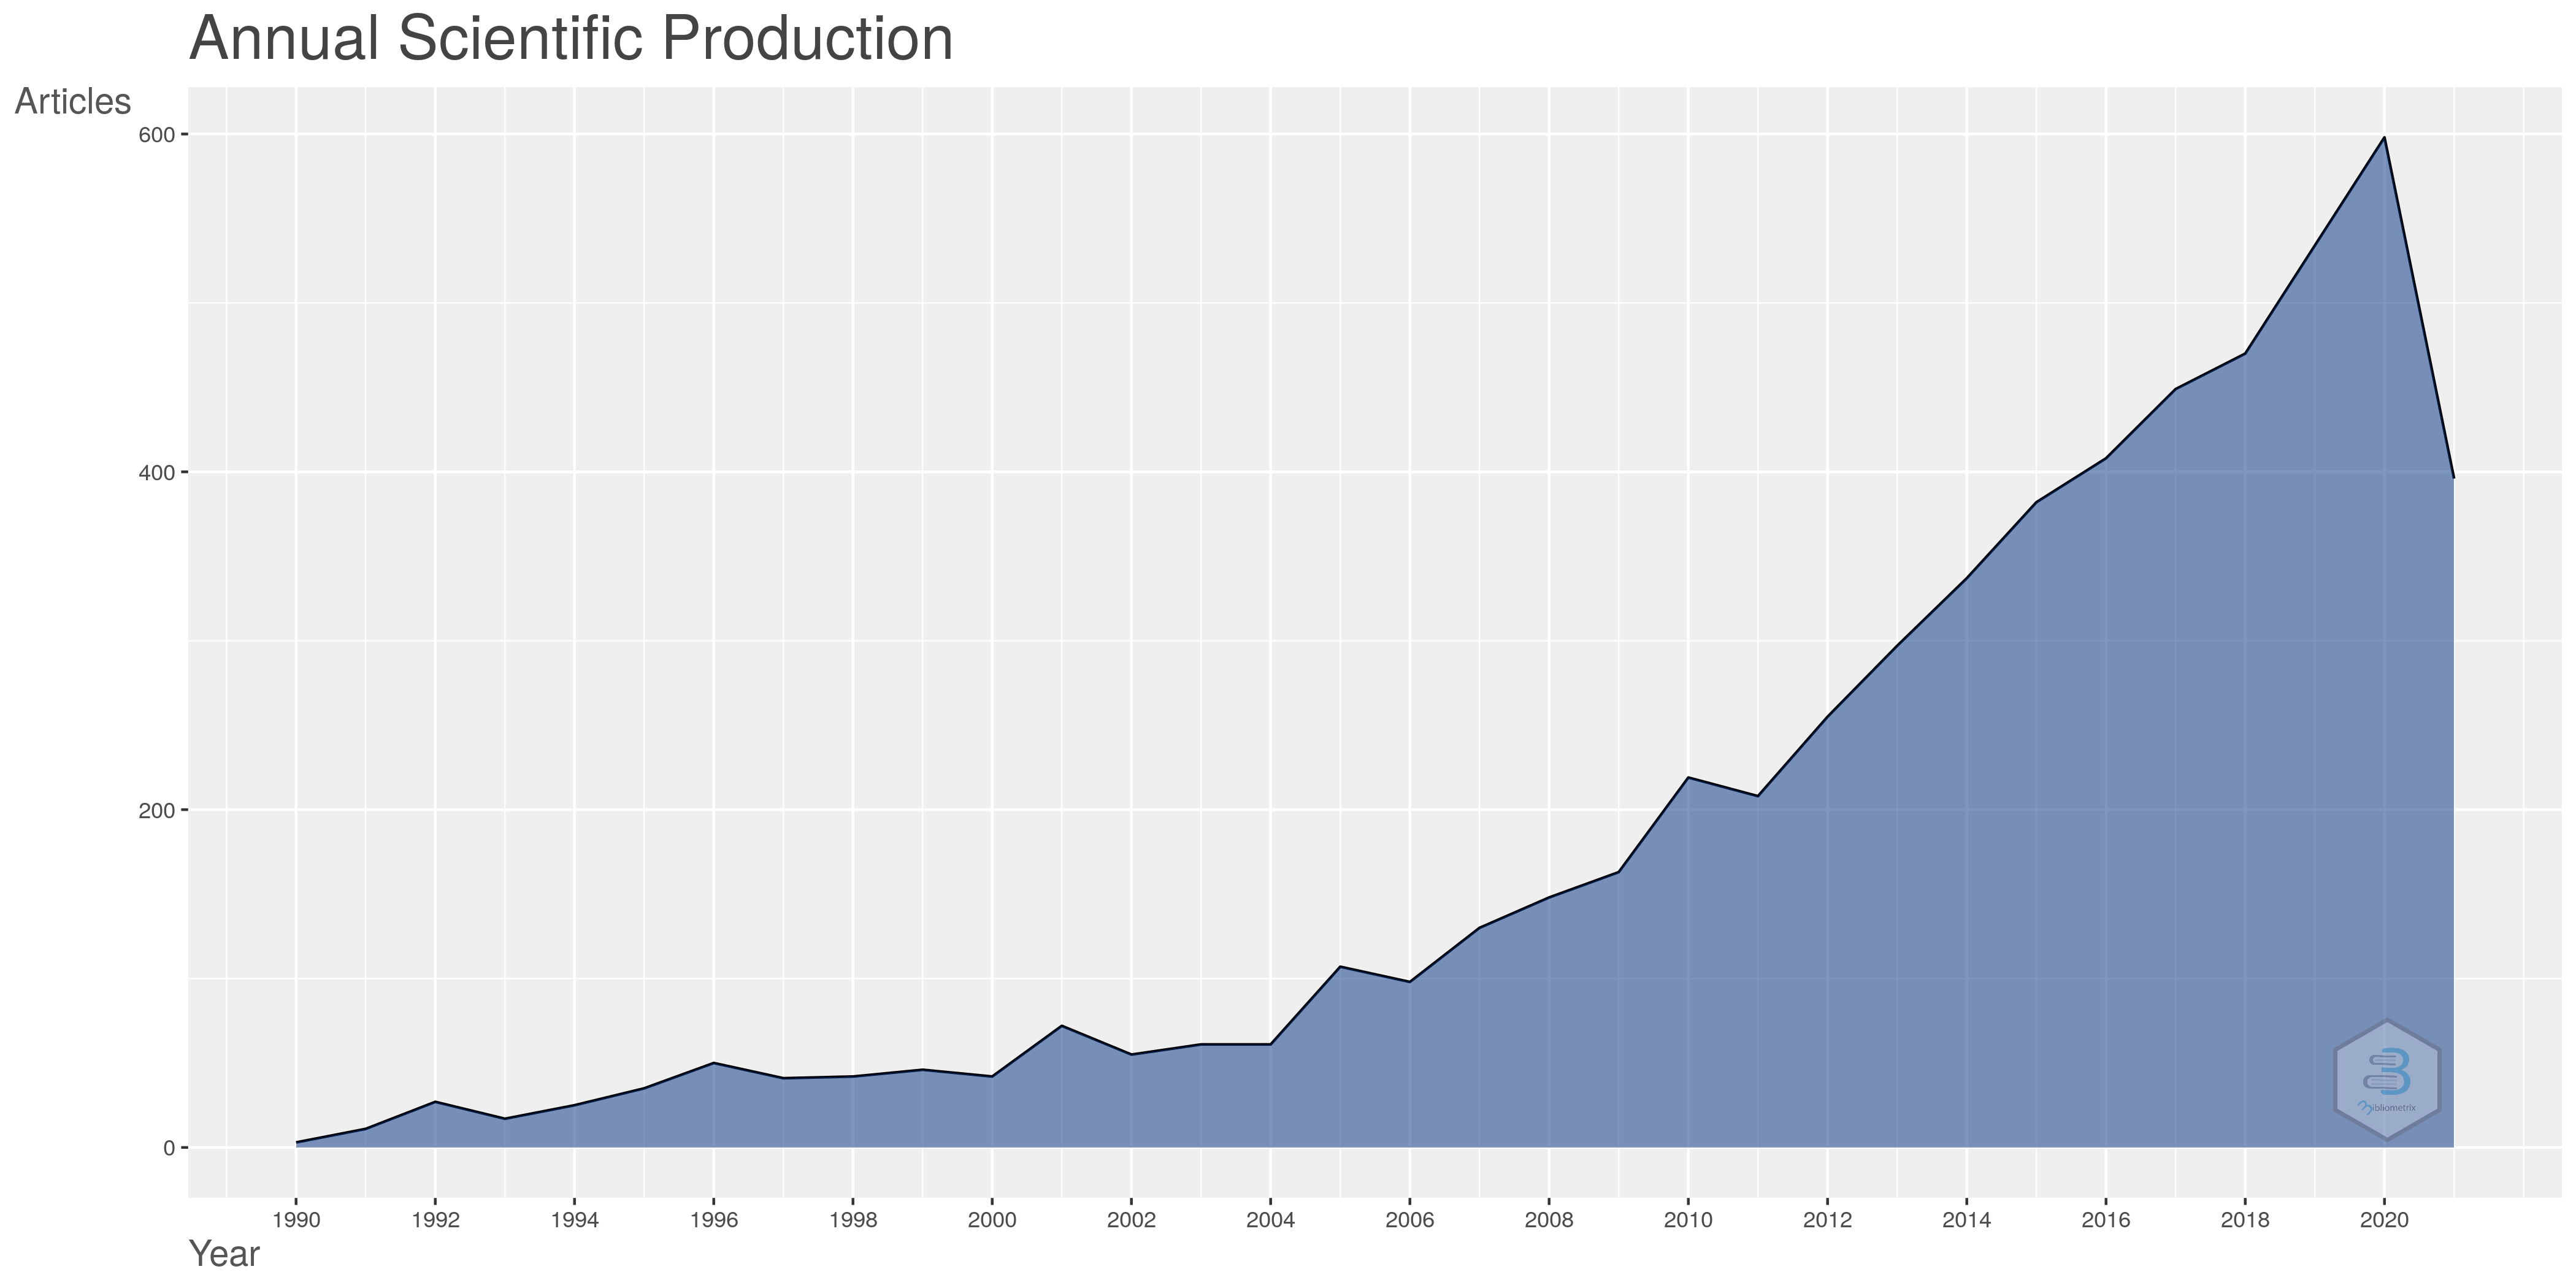
\includegraphics[width=1\textwidth]{experiments/jhcf/PesqBibliogr/Computacao Experimental/WoS-20210803/classico-mais-citacoes/Dataset/AnnualScientificProduction-2021-08-05.png}
    \caption{Evolução da produção científica no dataset MASSA@jhcf.}
    \label{fig:evol:anual:MASSA@jhcf}
\end{figure}

A figura \ref{fig:evol:anual:MASSA@jhcf} apresenta a evolução da produção científica mundial no tema de interesse, segundo o dataset MASSA@jhcf. A curva mostra uma tendência de crescimento aproximadamente exponencial da quantidade de publicações, desde a primeira identificada em 1990.

O \textit{Annual Growth Rate} do dataset é de 17,06\%, bem maior que a taxa média de crescimento da publicação científica mundial, de cerca de 3,3\% anuais, em 2016, como ilustra o estudo em \url{https://www.researchgate.net/publication/333972683_Dynamics_of_scientific_production_in_the_world_in_Europe_and_in_France_2000-2016}, página 23.

\subsection{Interpretação do Crescimento} A maior taxa de crescimento do dataset MASSA@jhcf, bem como o seu grande volume, sugerem que o assunto em pauta desperta intenso interesse, inclusive de ordem econômica.

\subsection{Evolução das Citações}

\begin{figure}
    \centering
    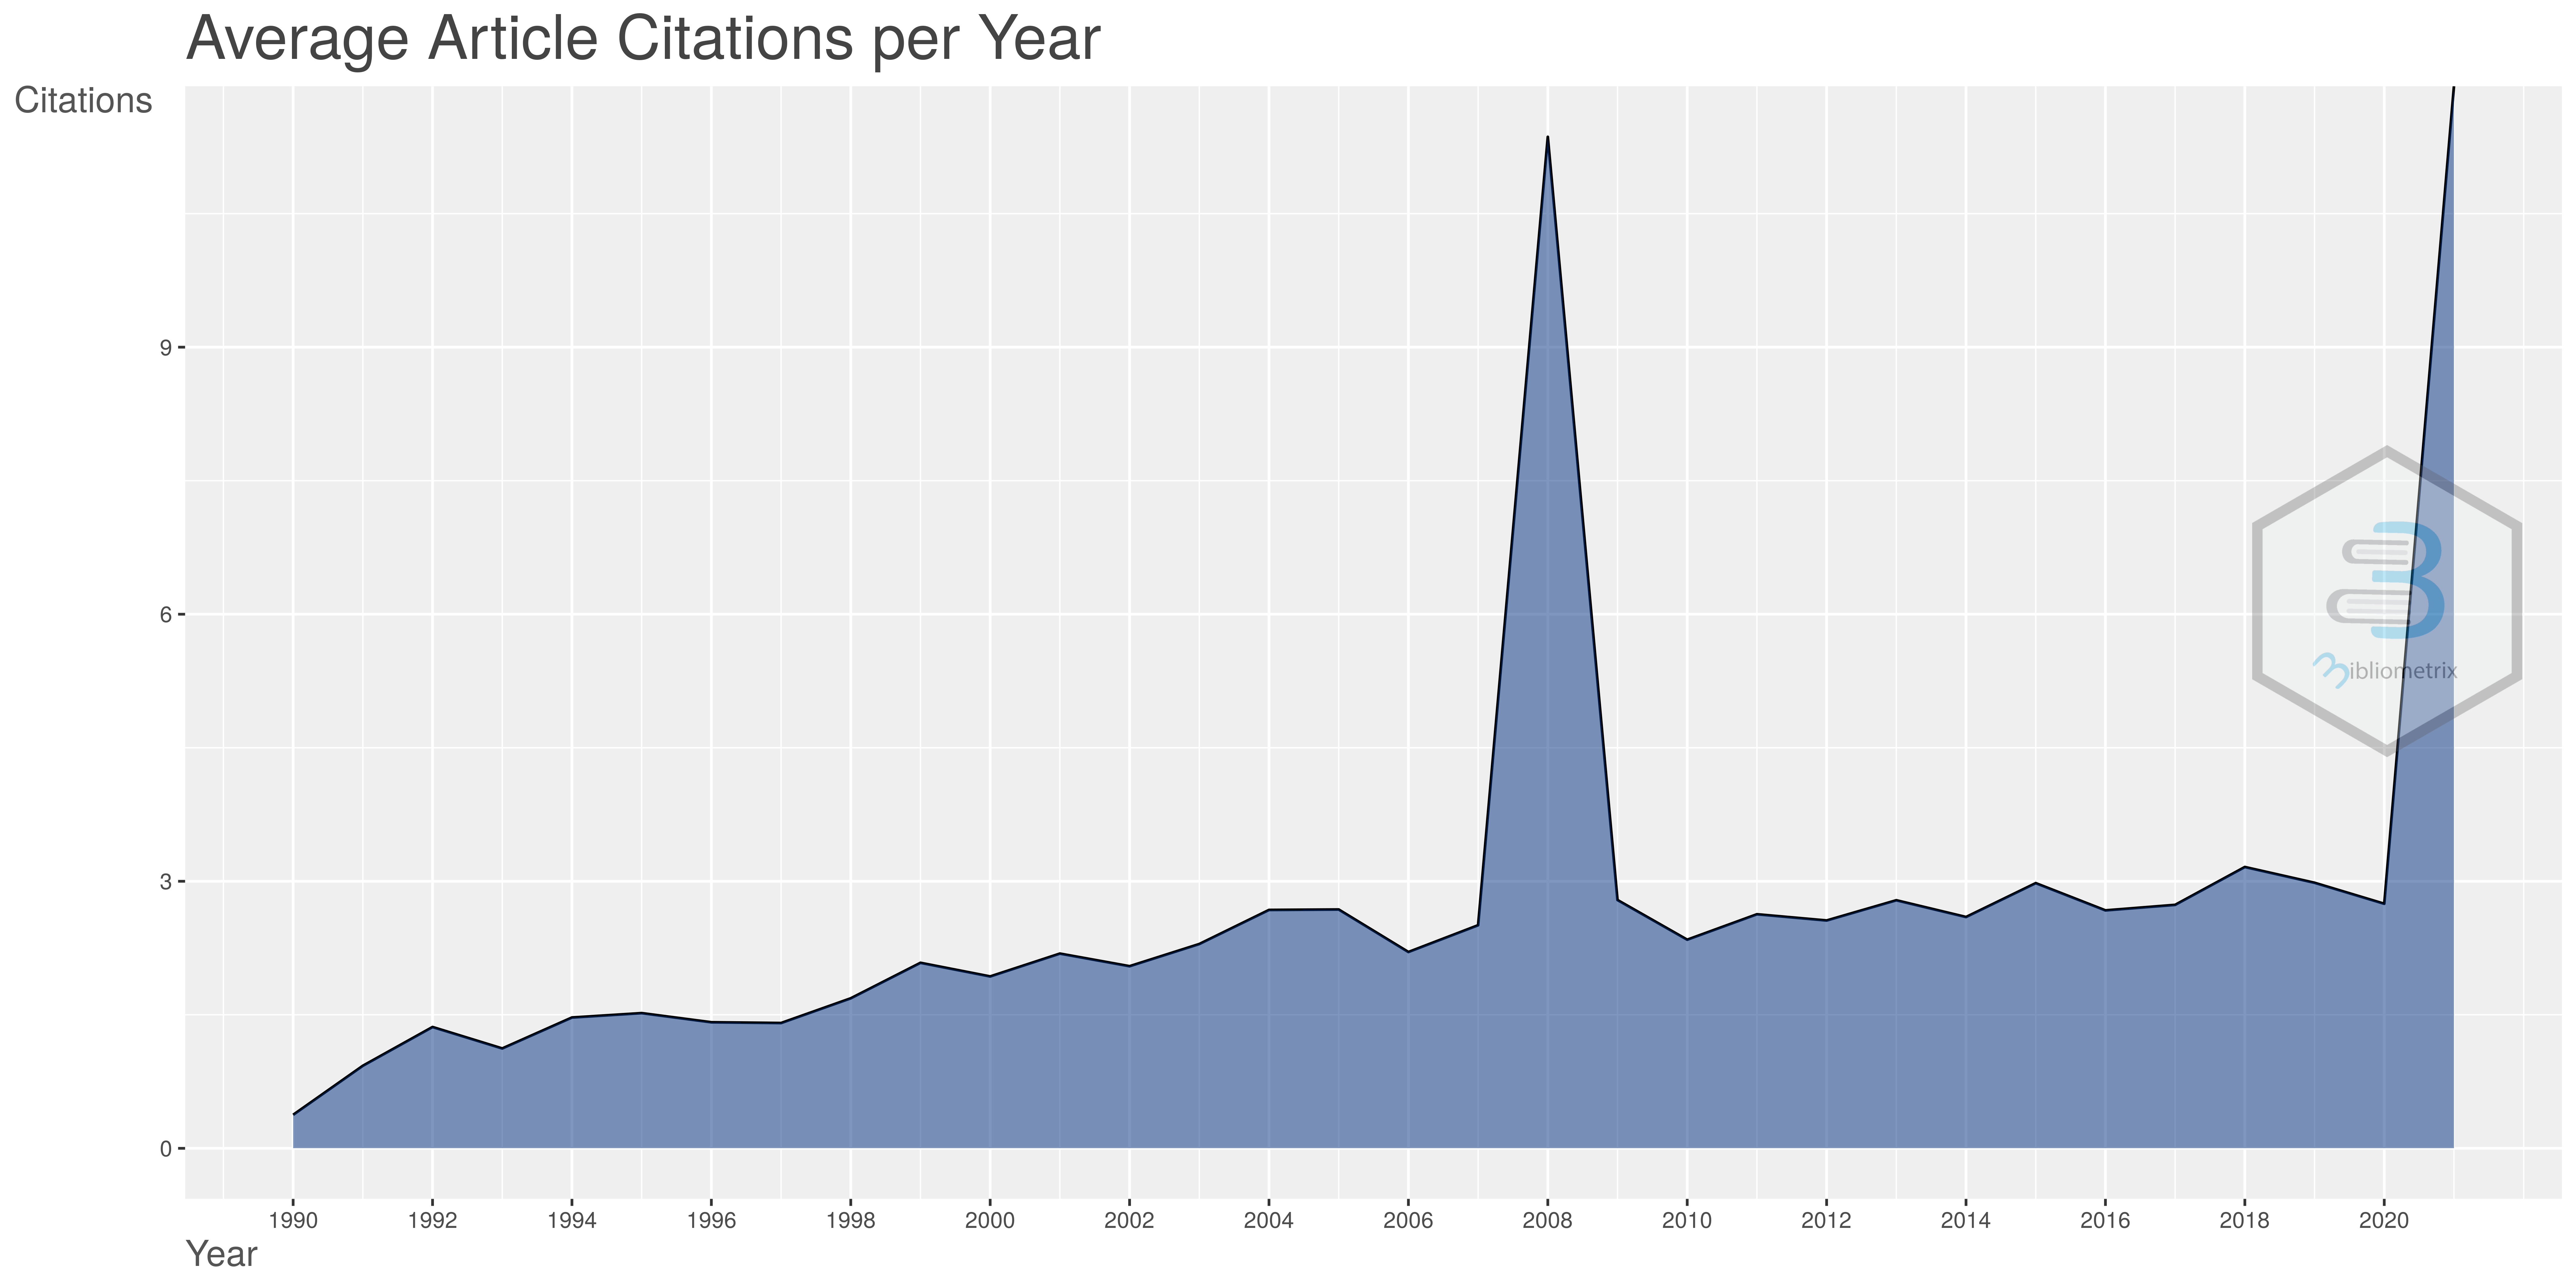
\includegraphics[width=1\textwidth]{experiments/jhcf/PesqBibliogr/Computacao Experimental/WoS-20210803/classico-mais-citacoes/Dataset/AverageArticleCitationPerYear-2021-08-09.png}
    \caption{Evolução das citações ao dataset MASSA@jhcf.}
    \label{fig:evol:anual:citacoes:MASSA@jhcf}
\end{figure}

A figura \ref{fig:evol:anual:citacoes:MASSA@jhcf} apresenta a evolução da média de citações aos 5.787 artigos no dataset MASSA@jhcf. 
Nota-se grande estabilidade na média anual de citações, onde os artigos publicados em 1992 possuem cerca de 2 citações médias, e em 2015 (17 anos depois) o valou alterou-se apenas para três. O pico que aparece no ano de 2008 deve-se, possivelmente, à presença de um artigo do dataset, publicado em 2008, que possui um número surpreendente grande de citações. \footnote{Note que o cálculo do número  médio de citações, nesse caso, utiliza os valores computados no tag "TC (Times Cited)", já presentes no dataset obtido. Ou seja, o gráfico baseia-se no número de citações globais (externas ao dataset MASSA@jhcf), e não no número de citações locais (citações a um artigo do dataset feitas por alguns dos outros artigos dentro do próprio dataset).}.

\subsection{Interpretação das Citações}
Mesmo perante um crescimento aproximadamente exponencial no volume de publicações, a ocorrência de um crescimento nas citações médias ao longo dos anos sugere que os artigos do dataset possuem uma tendência de crescimento no tamanho da bibliografia citada, bem como também despertam grande interesse dos cientistas nas demais áreas do conhecimento (já que se trata de citações globais).

\subsection{\textit{Three-Field Plots (Sankey diagram)}}

As \textit{Three-Field Plots (Sankey diagram)} (plotagens do tipo ``Três Campos'') apresentam afinidades entre três conjuntos de atributos agregados que ocorrem no dataset. Uma plotagem do tipo Sankey busca mostrar os principais fluxos entre diferentes conjuntos de itens. \footnote{Para uma introdução ver \url{https://en.wikipedia.org/wiki/Sankey_diagram}. Para obter detalhes sobre a forma de geração e utilização desse gráfico, inclusive de forma interativa, veja o vídeo em \url{https://www.youtube.com/watch?v=jBb1iha6-sg}.} 

\begin{figure}
    \centering
    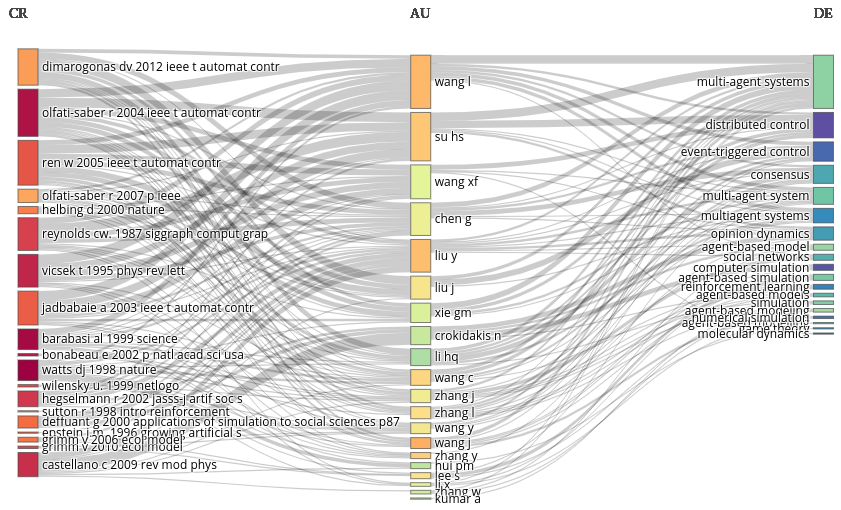
\includegraphics[angle=0,width=1\textwidth]{experiments/jhcf/PesqBibliogr/Computacao Experimental/WoS-20210803/classico-mais-citacoes/Dataset/ThreeFieldPlot-AU-CR-DE-20-20-20.png}
    \caption{Plotagem ``Três Campos'' (Sankey plot) do dataset MASSA@jhcf: 20 Autores, Citações e Palavras-Chave mais proeminentes.}
    \label{fig:MASSA@jhcf:ThreeFieldPlot}
\end{figure}

A figura \ref{fig:MASSA@jhcf:ThreeFieldPlot} apresenta a plotagem do tipo ``Três Campos'' do dataset MASSA@jhcf, vinculando, ao centro, os 20 Autores mais proeminentes (AU), à esquerda, as 20 Citações mais frequentes (CR - Cited Records), e à direita, as 20 Palavras-Chave mais frequentes empregadas pelos autores.

\subsection{Interpretação da figura \ref{fig:MASSA@jhcf:ThreeFieldPlot}}
Os vinte autores mais relevantes, em relação aos artigos mais relevantes citados, e as palavras-chave mais relevantes são aparentemente de origem asiática, mais especificamente chinesa, com base nos sobrenomes. De outra formal, a mesma origem chinesa parece não se aplicar aos trabalhos mais citados, aparentemente europeus ou norte-americanos. Isso sugere estar ocorrendo uma migração recente da produção científica, do ocidente para o oriente. 

Adicionalmente, dentre as palavras-chave (DE) não relacionadas diretamente aos termos de busca, emergem os termos \textbf{distributed control}, \textbf{event-triggered control}, \textbf{consensus} e \textbf{opinion dynamics}. Isso sugere foco das pesquisas por autores de origem chinesa no uso de simulação multiagente voltada à compreensão dos fenômenos de controle social distribuído, formação de consenso e dinâmica da opinião (pública?).

Ainda sobre a interpretação da plotagem da figura \ref{fig:MASSA@jhcf:ThreeFieldPlot}, observa-se que os artigos mais citados encontram-se publicados pelo menos 10 anos atrás, sugerindo que não houve, nos últimos 10 anos, nenhum trabalho que tenha produzido uma mudança de paradigma no tema.
A fim de melhor evidenciar as citações mais relevantes segundo o peso dos autores e palavras-chave, o gráfico da figura \ref{fig:MASSA@jhcf:ThreeFieldPlot:10-20-20} plota apenas as 10 referências citadas, para 20 autores e palavras-chave mais proeminentes.

\begin{figure}
    \centering
    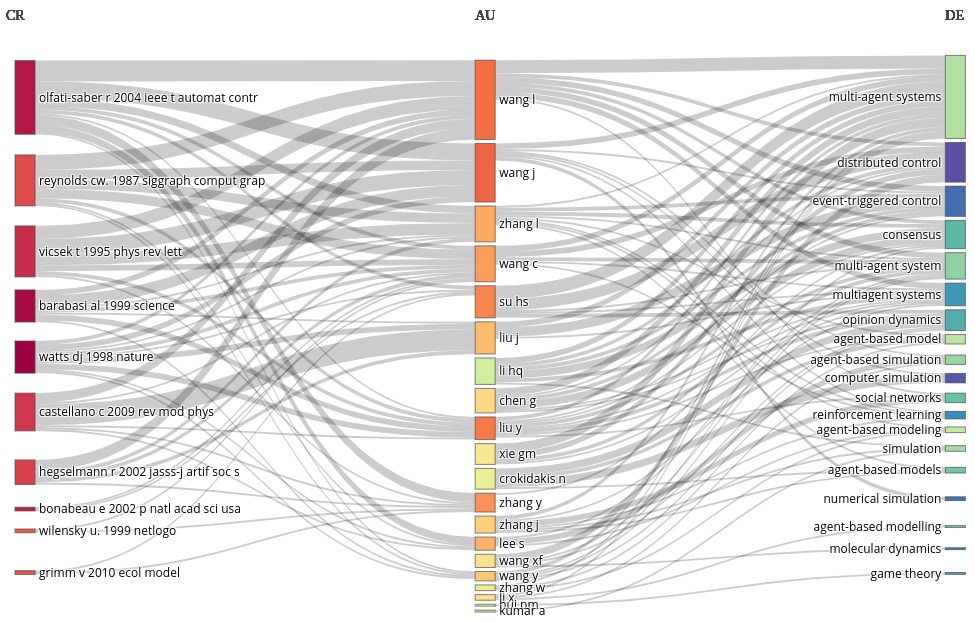
\includegraphics[angle=0,width=1\textwidth]{experiments/jhcf/PesqBibliogr/Computacao Experimental/WoS-20210803/classico-mais-citacoes/Dataset/ThreeFieldPlot-AU-CR-DE-20-10-20.png}
    \caption{Plotagem ``Três Campos'' (Sankey plot) do dataset MASSA@jhcf: 10 Autores, 20 Citações e Palavras-Chave mais proeminentes.}
    \label{fig:MASSA@jhcf:ThreeFieldPlot:10-20-20}
\end{figure}

Breves comentários sobre cada um desses trabalhos serão tratados em seção posterior.

\begin{itemize}
    \item  \cite{olfati-saber_consensus_2004} apresentam discussões teóricas sobre a formação de consenso em sistemas multi-agentes com topologias variáveis;
    \item  \cite{reynolds_flocks_1987} apresenta modelos multi-agentes para simulação gráfica do movimento de rebanhos ou agregados de animais.
    \item \cite{vicsek_novel_1995} analisam a emergência de fenômenos de transição de fase em simulações de de partículas com comportamento autônomo com interação biologicamente motivada.
    \item \cite{barabasi_emergence_1999} investigam a emergência da distribuição livre de escala (\textit{scale-free}\footnote{Ver introdução em \url{https://en.wikipedia.org/wiki/Scale-free_network}.}) em redes que evoluem com base em ligação preferencial.
    \item \cite{watts_collective_1998} exploram o surgimento de redes do tipo mundo pequeno (\textit{small world}\footnote{Ver introdução em \url{https://en.wikipedia.org/wiki/Small-world_network}.}) formadas a partir da reorganização aleatória de redes biológicas, genéticas e outras formas de redes auto-organizadas.
    \item \cite{castellano_statistical_2009} exploram de que forma as técnicas de análise e simulação já usadas na física-estatística podem ser usadas para explicar vários fenômenos sociais, tais como comportamento de multidões, dispersão social, comportamento de multidões etc. Eles apresentam as afinidades entre os dados gerados pelos modelos simulados e dados empíricos obtidos junto a sistemas sociais reais. 
    \item \cite{hegselmann_opinion_2002} exploram a emergência de fenômenos de consenso, polarização e fragmentação da opinião na simulação de sociedades artificiais.
    \item \cite{bonabeau_agent-based_2002} apresenta os potenciais e campos de aplicação da técnicas de simulação baseada em agentes.
    \item \cite{wilensky_netlogo_1999} apresentam a linguagem e ambiente de simulação NetLogo.
    \item \cite{grimm_standard_2006} apresenta o protocolo ODD, proposto para padronizar a descrição de modelos de simulação multiagente.
\end{itemize}

Nenhum desses 10 documentos citados está contido no dataset recuperado.

\subsection{Análises Bibliométricas: Fontes de Informação}

\begin{figure}
    \centering
%    \includegraphics[angle=0,width=1\textwidth]{}
    \caption{Plotagem ``Três Campos'' (Sankey plot) do dataset MASSA@jhcf: 20 Autores, Citações e Palavras-Chave mais proeminentes.}
    \label{fig:MASSA@jhcf:ThreeFieldPlot}
\end{figure}

\subsection{Análises Bibliométricas: Autores}

\subsection{Análises Bibliométricas: Documentos}



% \chapter{Análise Bibliográfica sobre \textit{Feedbacks} Automáticos no Ensino de Programação em Cursos de Graduação, por Fernanda Macedo de Sousa \label{chap:bibliometria:fernandams}}

\section{Planejamento do estudo}

% O planejamento o  desenho do estudo deve descrever as motivações, questões de interesse, escopo, limitações e objetivos do trabalho.

O ensino de programação nos anos iniciais das graduações tem sido um grande desafio didático e metodológico. Os ambientes Virtuais de aprendizagem (AVA’s) e demais plataformas de ensino emergem como possíveis soluções para sanar as dificuldades encontradas neste processo, porém a maioria destes ambientes não dispõe da dinamicidade necessária, que é intrínseca ao processo de ensino aprendizagem e, principalmente, ao ensino da primeira linguagem de programação. Neste contexto, o presente trabalho tem como intento responder à seguinte questão de pesquisa (RQ): O que nos diz a literatura sobre o uso de feedbacks automáticos no ensino de programação em cursos de graduação nas universidades de todo o mundo? A fim de responder ao RQ foram criadas 10 questões de investigação:

\begin{itemize}
    \item RQ1). Qual é a quantidade de artigos publicados por ano relacionados a este tema? 
    \item RQ2). Quais foram os países que mais produziram estes trabalhos? 
    \item RQ3). Quais fontes de informação publicaram mais artigos sobre esse tópico?
    \item RQ4). Quais são as principais plataformas de apoio ao ensino de programação utilizados atualmente?
    \item RQ5). Quais as principais linguagens de programação (Python, C, C++, Java, etc.) mais utilizadas no ensino da primeira linguagem de programação nos cursos de graduação?
    \item RQ6). Dentre os artigos analisados, qual a porcentagem dos que apresentaram resultados positivos em relação a implementação dos sistemas de feedbacks?
    \item RQ7). Estes feedbacks foram adaptados ao perfil do aluno ou são respostas padronizadas?
    \item RQ8). Os artigos analisados apresentaram alguma forma de classificação dos discentes por meio de suas respostas?
    \item RQ9). Os artigos apresentam alguma avaliação da percepção de quem faz uso dos feedbacks automáticos?
    \item RQ10). Qual o tipo de resposta apresentada nos feedbacks?
\end{itemize}

\subsection{O que já existe de pesquisa bibliométrica sobre esse tema?}

\subsection{Uso do Bibliometrix e Biblioshiny}
% Serão usadas a ferramenta e o \textit{workflow} proposto pelos autores do pacote Bibliometrix, conforme indica a figura ~\ref{fig:bibliometrix:workflow}.

\subsection{Limitações}

\section{Coleta de dados \label{FeedAuto:coleta}}

A coleta de dados foi realizada usando a base de dados Scopus no dia 09 de fevereiro de 2022, acessada por meio do Portal de Periódicos da CAPES.

Para a busca foram considerados os artigos publicados nos últimos cinco anos (2017 a 2021).

\subsection{Query de Busca}

Foi usada a \query\  de busca ilustrada nas linhas 1 a 14 da listagem \ref{query20220209-1}.

\lstinputlisting[numbers=left,basicstyle=\normalsize\ttfamily,caption={\query\  de busca sobre o uso de \textit{feedbacks} automáticos no ensino de programação em cursos de graduação},label=query20220209-1]
{experiments/fernandams/AnaliseBibliometrica/FeedbacksAutomaticosEnsProgGrad/Scopus-20220209/query.txt}

\subsubsection{Explicação para os termos de busca usados\label{FeedAuto:query}}

A busca consistiu de 

Os termos

\subsection{Registros recuperados}

\section{Análise dos dados}

\subsection{Filtragem de registros}

\subsection{Análise descritiva do \dataset\ FeedAuto@fernandams}

\subsection{Evolução da Produção Científica}

\subsection{Interpretação do Crescimento}

Percebe-se que esta é uma área de pesquisa em crescimento e que várias frentes de estudo estão sendo desenvolvidas em todo o mundo.

\subsection{Evolução das Citações}

\subsection{Interpretação das Citações}

\subsection{\textit{Three-Field Plots (Sankey diagram)} \label{FeedAuto:Sankey}}

\subsection{Interpretação da figura \ref{fig:FeedAuto@fernandams:ThreeFieldPlot}}

\subsubsection{Autores mais relevantes\label{FeedAuto:Sankey:AutoresRelevantes}}


\bibliographystyle{plainnat}
\bibliography{RESIC}

\end{document}.
